% LaTeX Template for short student reports.
% Citations should be in bibtex format and go in references.bib
\documentclass[a4paper, 9pt]{article}
\usepackage[top=3cm, bottom=3cm, left = 2cm, right = 2cm]{geometry} 
\geometry{a4paper} 
\usepackage[utf8]{inputenc}
\usepackage{textcomp}
\usepackage{graphicx} 
\usepackage{amsmath,amssymb}  
\usepackage{bm}  
\usepackage[pdftex,bookmarks,colorlinks,breaklinks]{hyperref}  
\hypersetup{linkcolor=black,citecolor=black,filecolor=black,urlcolor=black} % black links, for printed output
\usepackage{memhfixc} 
\usepackage{pdfsync}  
\usepackage{fancyhdr}
\usepackage{fancyvrb}
\usepackage{natbib}
\usepackage{url}
%\pagestyle{fancy}
\usepackage{tabto}
\usepackage[shortlabels]{enumitem}
\usepackage{tikz}
\usepackage{verbatim}
\usepackage{nameref}
\usepackage{caption}
\usepackage{subcaption}

\begin{document}
\graphicspath{{./Images/}}
\begin{flushleft}

\section*{Sardines: A Networked Game}

\textit{Sardines} is a system of communication for 2-8 players. Each player controls a submarine in real time, viewing their surroundings through the lens of a retro sonar system. These submarines communicate in morse code, firing soundwaves with thicknesses representative of dots and dashes to one another across the map. While this system has ultimately been designed for integration into a larger, more complete game, \textit{Sardines} presents itself as a sandbox, to best restrict attention to the networking techniques at play.

\subsection*{Architecture}\label{Architecture}

\textit{Sardines}' network uses a straightforward client-server architecture, with the server's `master' game state well-positioned to minimise disputes (see `\nameref{Prediction}'). Furthermore, the architecture uses local input processing - each client takes responsibility for processing their own player's actions and transmitting the resulting changes, rather than leaving the central server to compute a new master state directly from raw input. This distributes the game's physics-based movement calculations in a far more even fashion; an authoritative server with less trust in the player would better prevent cheating \citep{gmbta10}, but `cheating' will be of little concern while \textit{Sardines} remains a sandbox game.
%Reasons for choice...
%Though the current system does not have many variables to keep track of, the server also provides a `master state' for clients to work from.
%Citation about networking [peer-reviewed]...

\vspace{5pt}\noindent
\citeauthor{bauer04} \citeyearpar{bauer04} evaluate the scalability of this architecture, finding that with $n$ entity states (for the purposes of the report, players), client-server costs grow at order $O(n^2)$, compared to peer-to-peer's $O(n^3)$. They ultimately conclude that ``The client-server architecture exhibits the lowest growth in overall system cost, however, with the disadvantage that the entire growth must be handled by the central server.''  

\vspace{5pt}\noindent
In light of their findings, this report proposes a hybrid architecture for \textit{Sardines} to adopt at scale. While it ultimately proved too ambitious for this assignment, the original idea for the game was that \textit{multiple} players work together in piloting each submarine: a co-operative exercise with a navigator relaying key information about the surroundings, and a small team of other crewmates individually controlling acceleration, steering, etc. With only navigators witnessing the global game state first-hand, Figure \ref{Hybrid Architecture} positions these clients as `local' servers, processing (up to, say) $3$ players' inputs simulataneously, and relaying major changes to the game state back down to this crew. Not only does this topology require less of the central server's bandwidth (it still maintains $2$-$8$ connections, while each navigator has up to $4$ and other crewmates exactly $1$),  but demands far less calculation than if all $32$ players send their highly-individualised updates directly to the master state.

\vspace{0pt}\noindent
\begin{figure}[h]
\centering
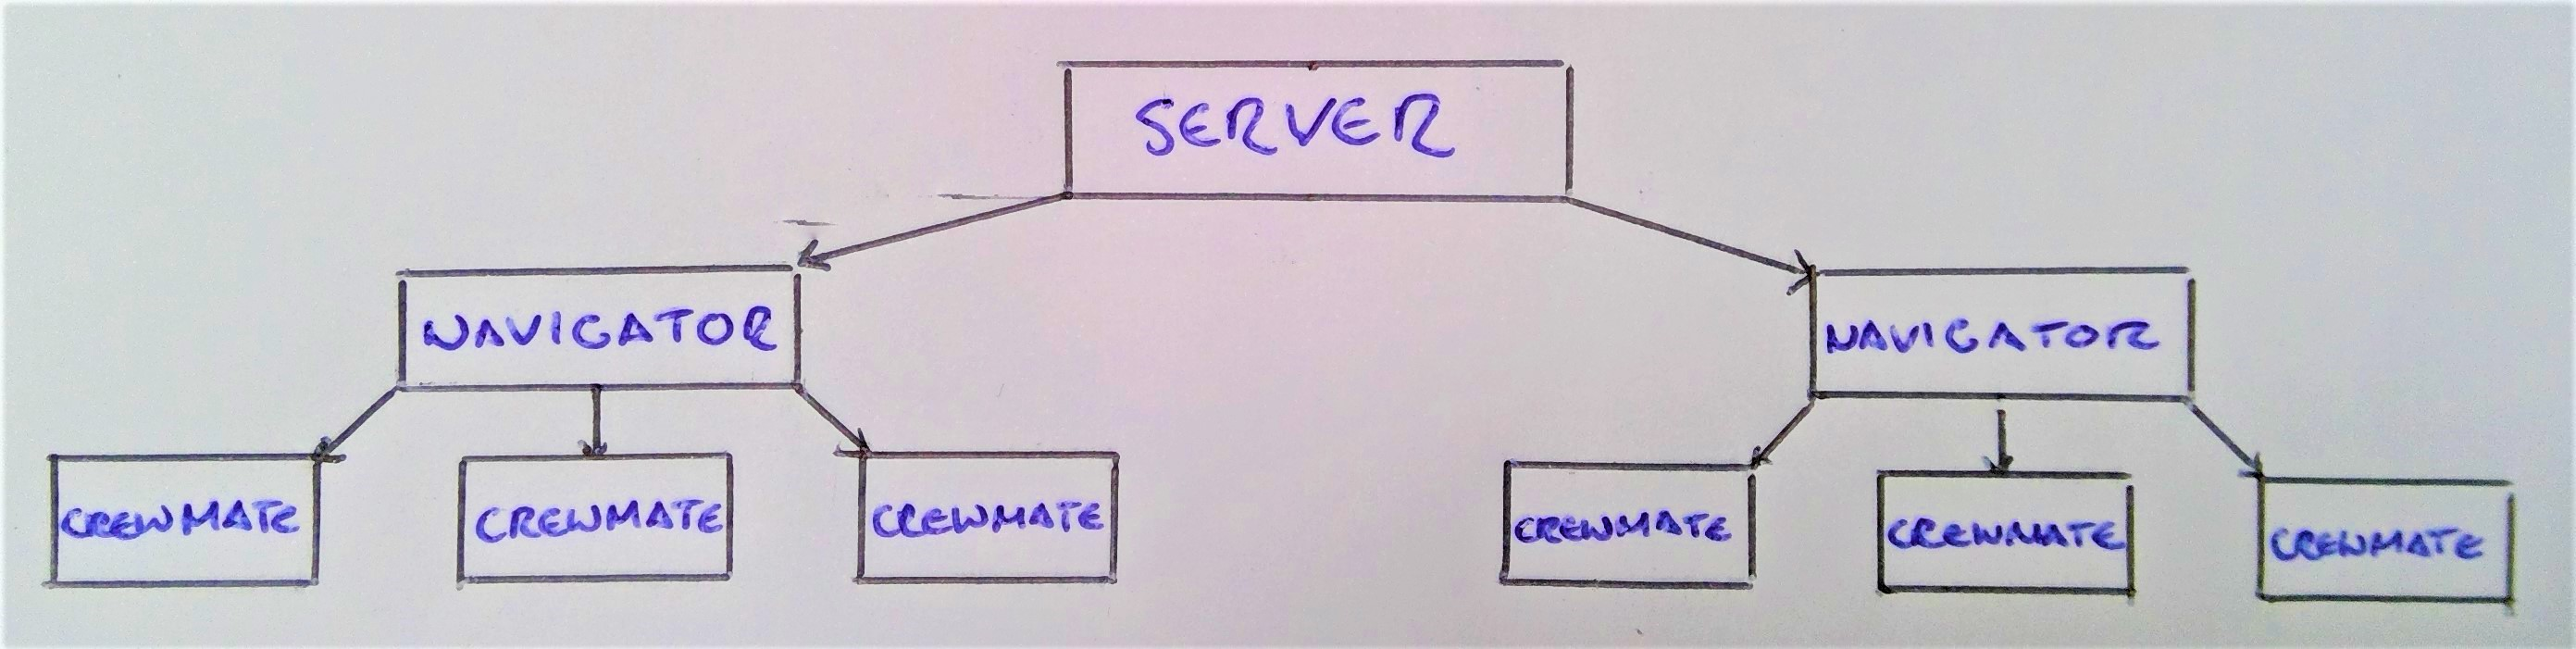
\includegraphics[width=0.75\textwidth]{Hybrid Architecture}
\caption{Potential hybrid architecture for a scaled version of \textit{Sardines}.}
\label{Hybrid Architecture}
\end{figure}

\subsection*{Protocols}\label{Protocols}

\paragraph{Transport Layer} In the application, client and server communicate through TCP connections, chosen for their robustness.
As described in RFC 798 \citeyearpar{rfc793}, where \citeauthor{rfc793} sets out the transport protocol,  %`` ''
\begin{quote}
Very few assumptions are made as to the reliability of the communication protocols below the TCP layer.  TCP assumes it can obtain a simple, potentially unreliable datagram service from the lower level protocols.  In principle, the TCP should be able to operate above a wide spectrum of communication systems.
\end{quote}
That the protocol guarantees reliability in-and-of-itself makes it perfect for \textit{Sardines}' purposes: for any two players to meaningfully communicate in morse code, they must be able to trust that their dots and dashes reach one another in order and without error.

\vspace{5pt}\noindent
There is, of course, an argument for updating positions via UDP. Suppose a submarine starts at point $A$, and fails to update to point $B$ - whereas a TCP connection will resend and resend this update until it succeeds, its ordered nature potentially holding up more important or immediate data, UDP assumes it \textit{has} sent correctly and moves on to the next point $C$. The minimalism of the protocol lends itself to the continuous, incremental nature of movement, but \textit{Sardines} will not make use of it. Submarines in this game travel slowly, with trajectories needed reliably but not immediately, and given a robust prediction system (see `\nameref{Prediction}') updating position via TCP every 0.2s should be infrequent enough to avoid the backlog described above.

\paragraph{Application Layer} 

While it needn't consider the internetwork and hardware layers of the protocol stack, the application layer of \textit{Sardines}' network necessarily interacts with the transport layer directly below it. Data is sent in a stream of \texttt{SendablePacket}s, consisting of a fixed-length \texttt{HeaderPacket} and one of several structs encoded as a \texttt{serialisedBody}. The header, always read first, contains a \texttt{bodyID}  that tells the receiver how many bytes of the body need deserialised; as discussed in the CMP501 labs, this application handles variable-length messages in much the same way as the DNS protocol.

\vspace{5pt}\noindent
At a more granular level, a \texttt{serialisedBody} may encode one of many structs, for one of many purposes:
\begin{itemize}[noitemsep]
\item \texttt{SyncPacket} Contains a \texttt{long} \texttt{syncTimestamp}. Sent on connection to estimate the travel time, \texttt{delay}, between client and server.
\item \texttt{IDPacket} Contains an \texttt{int} \texttt{clientID}, and a \texttt{char[]} \texttt{clientIP} that requires, by definition, no more than $16$ characters. Sent to initialise a client's unique identity, and let players track who else is playing.\footnote{In the hybrid architecture discussed above, the IP would also be used to establish crew-to-navigator connections.}
\item \texttt{SubmarinePacket} Contains an \texttt{int} \texttt{submarineID}, the controller's \texttt{clientID}, and additional variables for use in as-yet-unimplemented features. Similarly initialises a unique identity for each submarine.\footnote{And similarly, the distinction between \texttt{clientID} and \texttt{submarineID} is only meaningful with multiple clients per submarine.}
\item \texttt{PositionPacket} Contains a submarine's \texttt{x}-, \texttt{y}-coordinates and rotation \texttt{theta} at a certain time \texttt{timestamp}. Sent client-to-server as updates to the master game state, and server-to-client for prediction and rendering.
\item \texttt{MorsePacket} Similarly contains the necessary parameters to render a soundwave on the receiver's screen.
\item \texttt{EmptyPacket} Contains no variables. Sent when the \texttt{bodyID} corresponds to a function with no arguments (e.g. \texttt{bodyID} \texttt{2310} tells a server in lobby mode to initialise a game).
\end{itemize}
\texttt{bodyID}s adopt an informal naming convention: IDs \texttt{1XXX} refer to clients connecting to/disconnecting from a server, \texttt{2XXX} to server functionality while in lobby mode, \texttt{3XXX} to server functionality while in a game mode, and \texttt{4XXX} to client states and actions while in-game.

\vspace{5pt}\noindent
There isn't the space to break down every protocol in precise detail, but all have been designed with the same underlying philosophy. Consider, for instance, the process of joining a lobby:
\begin{enumerate}[label=\textit{\arabic*}\textit{.}, noitemsep]
\item \textit{The client registers a TCP connection with the server, and sends a \texttt{syncPacket} (ID \texttt{1000}).} %The client then constructs a \texttt{syncPacket} (ID \texttt{1000}) to send over the connection.
\item \textit{The server receives a \texttt{SyncPacket} from the client, and returns it, via \texttt{Receive1000()}.} %Calling \texttt{Receive1000()}, the server returns its own \texttt{syncPacket}, with \texttt{syncTimestamp} set to the timestamp on the received \texttt{HeaderPacket}.
\item \textit{The client receives a \texttt{SyncPacket} from the server, estimates travel time between the two devices, and sends an \texttt{IDPacket} (ID \texttt{1001}), via} the client version of \textit{\texttt{Receive1000()}.} %With its own version of \texttt{Receive1000()}, the client uses the packet to estimate the time difference with the server. An \texttt{IDPacket} (ID \texttt{1001}) is then sent to confirm the player's identity.
\item \textit{The server receives an \texttt{IDPacket} from the client, changes the \texttt{clientID} if it is unrecognised,\footnote{Or banned! In this case, the server returns an \texttt{IDPacket} with a strictly negative \texttt{clientID}, which cues the client to disconnect.} and returns it, via \texttt{Receive1001()}.} %If it recognises the received \texttt{clientID}, \texttt{Receive1001()} returns it unchanged; if it is unrecognised, it returns a newly-assigned identity.\footnote{And if, for any reason, the player is recognised as banned from the server, it will return a strictly negative \texttt{clientID} that the client takes as its cue to disconnect!} % (or, to reject the client, returns the packet with \texttt{clientID} set to \texttt{-1}).
\item \textit{The client receives an \texttt{IDPacket} from the server, a formal acceptance into the lobby, via \texttt{Receive1001()}.} %The client adopts the returned \texttt{clientID}, taking this as a `formal' acceptance onto the server.
\item \textit{All clients receive (further) \texttt{IDPacket}s from the server (IDs \texttt{1002}). These tell players in the lobby who has just joined, and vice versa, all via \texttt{Receive1002()}.}
\end{enumerate}
The process is designed for ease of programming: treating major protocols as a chain of smaller, simpler steps, it becomes far easier to manage - and document - the application layer (even if there is some unnecessary back-and-forth to the above).
%This description may seem fairly dry, but it serves to ...
%There is some degree of back-and-forth to this process...


\subsection*{API}

% CHECKME: What is an API?
\textit{Sardines} is written in C\#, for the Godot engine. It uses System.Net.Sockets to handle networking, and System.Runtime.InteropServices to serialize/deserialize packet structs. As noted in the documentation \citeyearpar{msftSNS}, System.Net.Sockets implements conventional Berkeley sockets.

\subsection*{Integration}

Each client organises its networking components in a \texttt{Handler} class, along with a `local' copy of the game state. This is treated as a black box by the game at large, with local processing entered in and external updates read back out. Consider, for example, how the \texttt{NavigationDisplay} interacts with the \texttt{Handler}. Every frame, \texttt{UpdatePosition()} pushes the player's new position into the local state and sends it on to the server; then, \texttt{Render()} pulls that same data in displaying (a relative view of) their surroundings onscreen.

\vspace{5pt}\noindent
Client and server communicate `as and when'. Since TCP connections risk blocking either component, both rely on I/O multiplexing. The server uses System.Net.Sockets' \texttt{select()} function to monitor all connections simultaneously, set to time out after $1ms$. Each client does the same with its single server connection, to avoid freezing the broader game - \texttt{select()} will still block, however, sometimes resulting in an unfortunate buffering effect under poorer network conditions.\footnote{In hindsight, the function should have been set to time out immediately, at \texttt{0}.}

\subsection*{Prediction}\label{Prediction}

As discussed in `\nameref{Protocols}',  clients only send position updates every $0.2s$. What this report has so far failed to consider is how this appears to other clients - they experience what should be a smooth, continuous movement as discontinuous jumps over $0.2s$ intervals! \textit{Sardines} resolves this with a combination of techniques.

\vspace{5pt}\noindent
When players choose to move forward, they do not jump to a constant speed but slowly ramp up from zero; the game makes a second-order, quadratic prediction to best approximate the second-order derivative that is acceleration. Given a submarine's three most recent positions $\mathbf{r}_0$, $\mathbf{r}_1$, $\mathbf{r}_2$ (corresponding to times $t_0 > t_1 > t_2$), clients can average the velocities from $\mathbf{r}_1$ to $\mathbf{r}_0$, from $\mathbf{r}_2$ to $\mathbf{r}_1$, and the acceleration from $\mathbf{r}_1$ to $\mathbf{r}_0$ as
$$\mathbf{u}_0 = \frac{\mathbf{r}_0-\mathbf{r}_1}{t_0-t_1}, \;\; \mathbf{u}_1 = \frac{\mathbf{r}_1-\mathbf{r}_2}{t_1-t_2}, \;\; \mathbf{a}_0 = \frac{\mathbf{u}_0-\mathbf{u}_1}{t_0-t_1}, \;\; \textrm{respectively.}$$
These parameters define the quadratic model
$$ \mathbf{\tilde{r}}(t) = \mathbf{r}_0+\mathbf{u}_0t+\frac{1}{2}\mathbf{a}_0t^2.$$
%FIXME: Subject to experiementation!
In contrast, the rudder controlling a submarine's rotation $\theta$ \textit{does} move at a constant speed, so \textit{Sardines} only uses linear prediction to approximate
$$\mathbf{\tilde{\theta}}(t) = \mathbf{\theta}_0+\mathbf{\dot{\theta}}_0t$$
(taking extra care to handle jumps from $\theta \approx 0$ to $\theta \approx 2\pi$, and vice versa).


\vspace{5pt}\noindent
If prediction is how one waits for data, then integration is what one does on its arrival. Receiving a new \texttt{PositionPacket} at time $t_0$, a programmer may wish to switch to new quadratic model $\mathbf{\tilde{r}}_{\textrm{new}}(t)$ immediately, but if positions $\mathbf{\tilde{r}}_{\textrm{old}}(t_0)$ and $\mathbf{\tilde{r}}_{\textrm{new}}(t_0)$ are visibly far apart then the player will see the corresponding submarine make an instantaneous jump across the screen.\footnote{This might be regarded as interpolation over $T = 0.0s$!} Instead, one takes a set time $T$ to linearly interpolate from the old trajectory to the new:
$$\mathbf{\tilde{r}}(t) = \begin{cases} 
\mathbf{\tilde{r}}_{\textrm{old}}(t) & \textrm{if $t < t_0$} \\
(1-q(t))\mathbf{\tilde{r}}_{\textrm{old}}(t) + q(t)\mathbf{\tilde{r}}_{\textrm{new}}(t) & \textrm{if $t_0 \leq t < t_0+T$} \\
\mathbf{\tilde{r}}_{\textrm{new}}(t) & \textrm{if $t \geq t_0+T$}
\end{cases}, \;\; \textrm{where $q(t) = \frac{1}{T}\left(t-t_0\right)$.}$$
In \textit{Sardines}' particular implementation, \texttt{PositionPacket}s are sent via TCP every $0.2s$; interpolation therefore takes place over a strictly shorter interval $T = 0.1s$. 
%Footnote - quirk of how we deal with being two packets behind?

\begin{figure}[h]
\centering
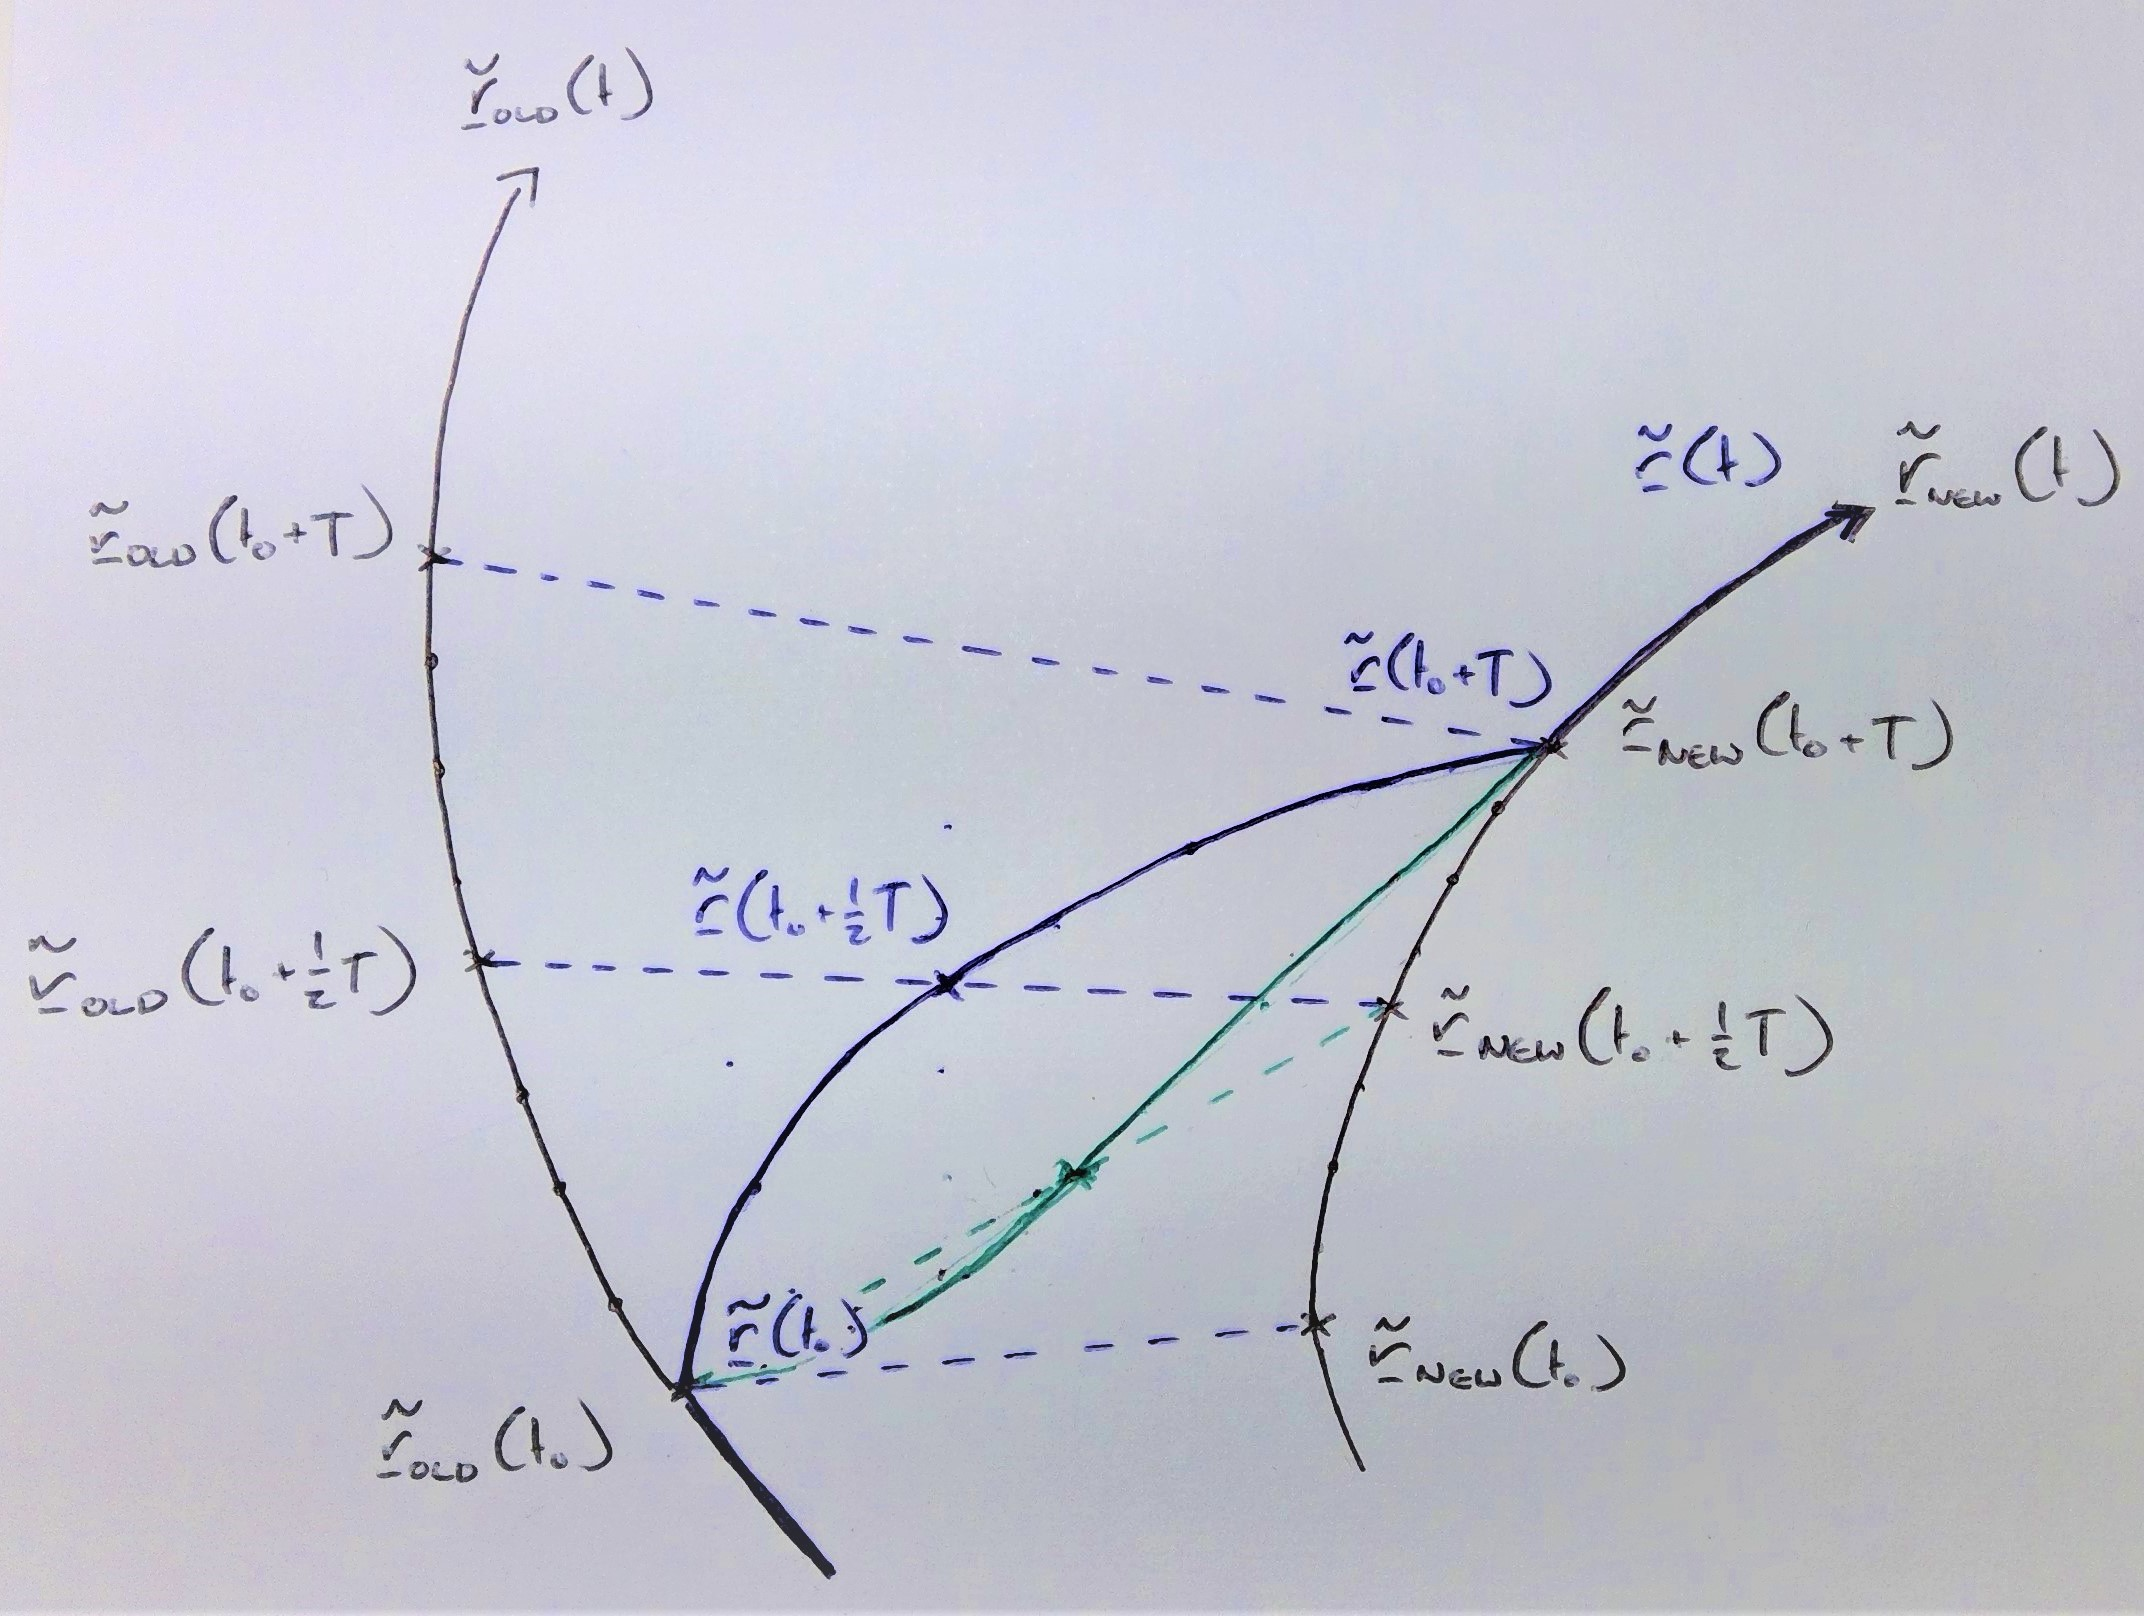
\includegraphics[width=0.85\textwidth]{Interpolation}
\caption{Interpolation from trajectory $\mathbf{\tilde{r}}_{\textrm{old}}(t)$ to $\mathbf{\tilde{r}}_{\textrm{new}}(t)$ (blue); chosen over $\mathbf{\tilde{r}}_{\textrm{old}}(t_0)$ to $\mathbf{\tilde{r}}_{\textrm{new}}(t)$ (green).}
\label{Interpolation}
\end{figure}

\vspace{5pt}\noindent
A classic problem in networked game design is one of conflict resolution - if client $A$ hits client $B$ with a projectile in their own local state, but misses in $B$'s, whose account does the server take as true? In \textit{Sardines}, the projectiles concerned are soundwaves. The visual language of the game, where waves from external sources only become visible on collision with the player, provides a clear approach: the sender unequivocally takes precedence. Only when a player sees their soundwave hit another is a \texttt{MorsePacket} sent from their client (which will arrive with the usual delay). The sender knows with certainty who receives their message; the receiver, who cannot see the trajectory of the soundwave until it arrives, will have no sense whether it `should' have hit them according to their local game state.

\vspace{5pt}\noindent
To further smooth over the application's disputes, the receiving client makes use of backward prediction. Since neither server nor client stores more than three of any submarine's past positions at a time, it is fortunate the above definition of $\mathbf{\tilde{r}}(t)$ can approximate the past as well as the future.\footnote{\textit{Sardines}' submarines are physics-based objects, and at one point in development, the drag they experience was factored into prediction. However, the differential equations for 2D motion with a quadratic drag were too complex to find an analytic solution - rather than being able to substitute a $t$-value into a given equation, the prediction would be calculated over incremental, irreversible forward time steps - so the application sacrifices this more realistic model for the ability to look backwards in time.}

\vspace{5pt}\noindent
Suppose a sender emits a soundwave from position $\mathbf{r}$ at time $t_0$, which they see reach a receiver at $t_0+\Delta t$. On the arrival of the corresponding packet at $t_1$, then, the receiving client has to decide where the wave was emitted from \textit{in its local view of the game}. The obvious choice would be the `true origin' $\mathbf{r}$, but \textit{Sardines} uses the backwards prediction $\mathbf{\tilde{r}}(t_1-\Delta t)$. Conflict resolution is, fundamentally, the art of deciding which quantities are preserved across clients, and \textit{Sardines} - a system exploring slow, real-time communications - is far less concerned with presenting a shared view of geography than it is a shared view of delay.

\subsection*{Testing}\label{Testing}

\vspace{5pt}\noindent
The following insights are made with the help of clumsy. %\footnote{Note that - with testing so integrated into the larger development process - the clients tested were often run within the Godot editor. With poorer performance than a standalone executable, the following results may constitute more of a worst-case scenario for \textit{Sardines} than intended...} 
This tool can simulate many a real-world network condition, but in the interests of brevity the section will restrict its attention to two most relevant to the TCP-based game at hand: latency (where all data are delayed by a set interval) and throttle (where data over a set interval are held back, then sent all at once).

\paragraph{Latency} While opinions will vary on what consistutes a `reasonable' amount of lag, \textit{Sardines} shows promise. The predictions made here provide a smooth enough experience at a latency of $200ms$, even $250ms$, with the game only becoming unplayable at higher thresholds. A latency of, say, $500ms$, will see the clients' worldviews slowly desynchronise, accumulating more and more error as time goes on. With no immediate solution in sight, one might be inclined to take a step back, and interrogate the network's more basic assumptions; it could well be that the theory behind, say, eschewing UDP connections has not held up in practice...%Though it cannot yet identify the cause of this desynchronisation effect, the report offers an optimistic outlook - %so much of network programming %one of the most valuable lessons of this whole assignment has been that, when faced with a seemingly-inexplicable bug, it is always worth taking a step back and re-evaluating the assumptions the network makes.%This desynchronisation bug appears a barrier to further success, the cause of which is unidentified - having come across such error 


\vspace{5pt}\noindent
At any rate, there are more concrete fixes that can be made before worrying about such an open-ended performance issue - consider, for instance, how travel times are calculated between client and server. Currently, \texttt{delay} is averaged from $5$ \texttt{syncPacket}s sent back and forth immediately on joining a lobby, which comes with a slow loading time but results in (initially) accurate predictions. What this implementation misses is how \texttt{delay}s may vary over larger time scales; the experience of testing latency and realising how travel times can be affected by lag spikes suggests these values should be recalculated at least semi-regularly. %In theory, it is enough to average over a small sample of these times immediately on joining a lobby, but the experience of testing latency suggests this value could ebb and flow over a larger timescale. Recalculating...


\begin{figure}[h]
\centering
\begin{subfigure}[b]{0.3\textwidth}
\centering
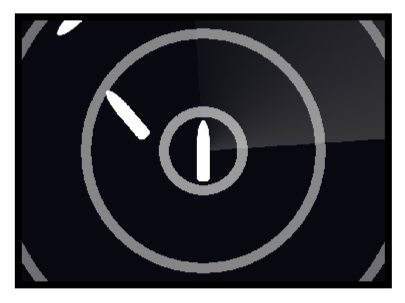
\includegraphics[width=\textwidth]{100ms Latency (0)}
\end{subfigure}
\centering
\begin{subfigure}[b]{0.3\textwidth}
\centering
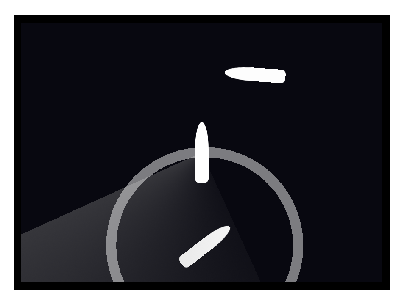
\includegraphics[width=\textwidth]{100ms Latency (2)}
\end{subfigure}
\centering
\begin{subfigure}[b]{0.3\textwidth}
\centering

\includegraphics[width=\textwidth]{100ms Latency (1)}
\end{subfigure}
\caption{Three simultaneous, local views of the game world, at $100ms$ latency (taken during development). These positions would appear consistent, in spite of the delay.}
\label{Lag Testing}
\end{figure}

\paragraph{Throttle} On one hand, \textit{Sardines} would appear to have a built-in tolerance for throttle. Of all the variables in the application layer, clients only update position values continuously, and only when those position values are actively changing - and only \textit{then} once every $0.2s$. It is therefore unsurprising that using clumsy to simulate $<200ms$ throttle (with probability $10\%$) has little visible effect. However, with values just above this again giving way to desynchronisation,\footnote{Similarly - the application can't even handle a $5\%$ packet loss...} the attached video demostrates performance at $300ms$ latency, with a $10\%$ chance of $200ms$ throttle. This is a set of poor network conditions chosen to best challenge the application, without breaking it altogether.%since it only . %For these reasons, the video demonstration : it is 


%Testing lag and throttle simultaneously yields unsurprising results. Having established acceptable network conditions - [TIME]$ms$ lag, a [$\%$ chance of [TIME]$ms$ throttle -

\vspace{5pt}\noindent
Recall the interpolation technique described above. Since $T < 0.2s$, the report has assumed the submarine being interpolated starts on a predicted trajectory at time $t_0$ - does this assumption hold in practice? If two \texttt{PositionPacket}s have been throttled, and arrive within $T$ seconds of each other, it follows that the submarine will not have finished its first interpolation by the time the second one begins. In this edge case of being caught mid-interpolation at some point $\mathbf{r}_0$, \textit{Sardines} prioritises catching up; rather than using a predicted trajectory as in Figure \ref{Interpolation}, the subsequent interpolation simplifies calculations by taking $\mathbf{\tilde{r}}_{\textrm{old}}(t) = \mathbf{r}_0$.

\vspace{5pt}\noindent
Other issues remain unresolved in the submitted application, one being a vulnerability in the clients' morse code. While it's true that a TCP connection will preserve the order of dots and dashes, it will not preserve the intervals at which they were sent - if two or more throttled soundwaves end up showing at the same time, their order becomes indistinguishable! These could easily be staggered by a simple `queuing system' on the receiver's end.
%Whether this is resolved by a straightforward queueing system, or a more general revamp of the entire mechanic, this represents a rare case where the game's design is 

\vspace{5pt}\noindent
For all the optimisations and oversights discussed above, it's worth noting how fundamental testing has already been to development. With network programming being notoriously unpredictable, \textit{Sardines} has necessarily involved a lot of quality assurance: a feature that works offline must be tested between a single client and the server; then between two clients on the same device; then across devices, or between more clients, or under poor network conditions; the list goes on. This section takes a largely qualitative approach in order to reflect the role of clumsy in this process, as a means to poke and prod at the underlying network. \textit{Sardines} is not, in the end, a perfect application. The goal of this report is not to obscure its flaws, but to better understand them.
%To conclude
%While this report cannot yet explain that earlier issue of desynchronisation, it can absolutely offer lines of attack - be that re-examining [Conclude here, or one final paragraph for more general reflection?]. 

\bibliographystyle{agsm}
\bibliography{References}
\end{flushleft}
\end{document}

